\documentclass[border=10pt]{standalone}
\usepackage{tikz}
\usetikzlibrary{arrows.meta, shadows.blur, backgrounds, calc, decorations.pathmorphing}
\usepackage{amsmath}
\begin{document}
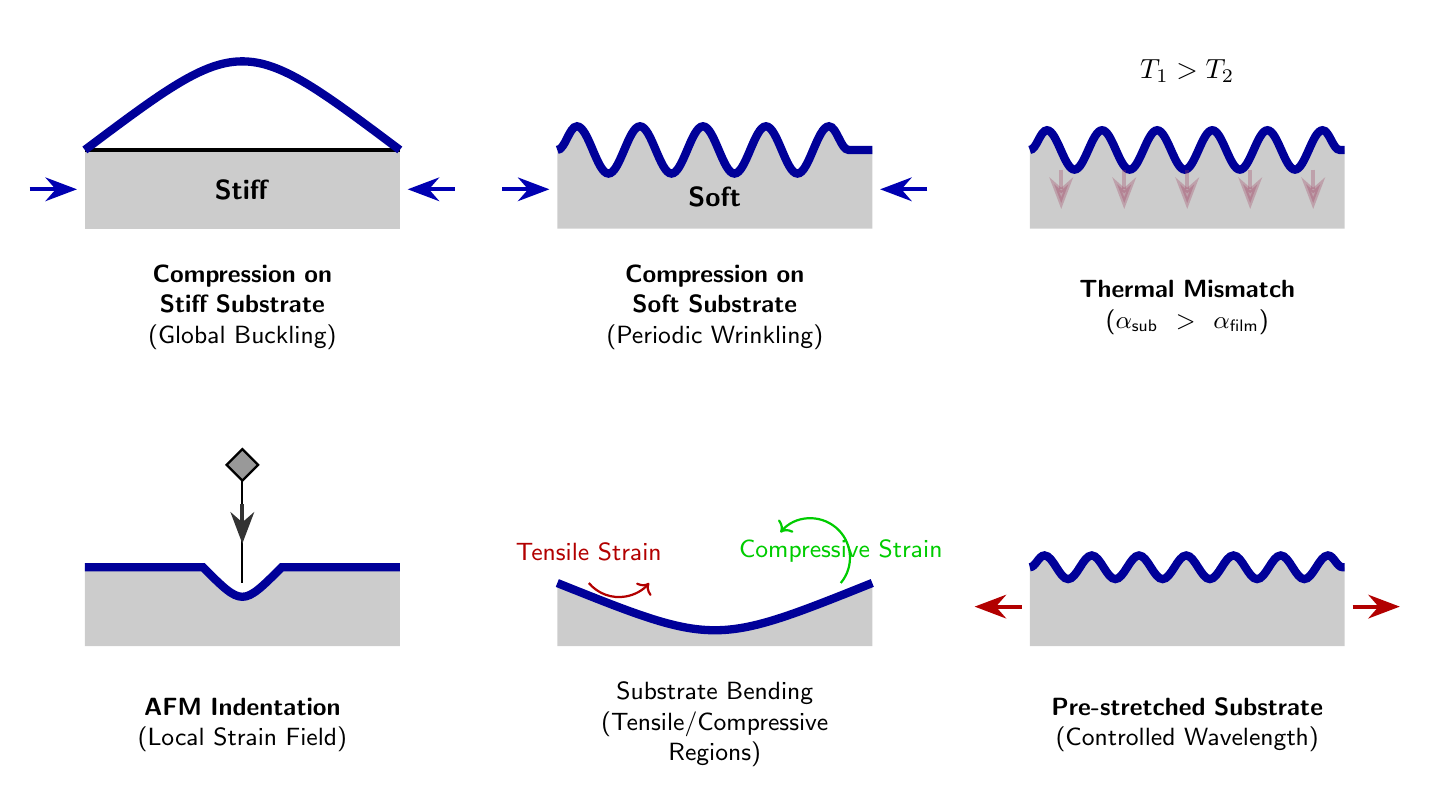
\begin{tikzpicture}[font=\sffamily\bfseries]

  % Define updated styles
  \tikzset{
    substrate/.style={fill=gray!40},
    topline/.style={draw=black, line width=1.5pt},
    tmd/.style={
      draw=blue!60!black,
      top color=white,
      bottom color=white,
      shading=axis,
      shading angle=90,
      line width=2pt,
      drop shadow={shadow xshift=0pt,shadow yshift=-1pt,opacity=0.2}
    },
    arrow/.style args={#1}{-{Stealth[length=4mm,width=3mm]},line width=1.5pt,color=#1},
    panel label/.style={font=\sffamily\small,align=center,text width=4cm},
    title/.style={font=\sffamily\bfseries\large},
    summary/.style={font=\sffamily\small,align=left,text width=11cm}
  }

%% Panel 1: Global Buckling with "Stiff" inside
\begin{scope}[shift={(-6,2.8)}]
  \fill[substrate] (-2,-0.5) rectangle (2,-1.5);
  \draw[topline] (-2,-0.5) -- (2,-0.5);
  \draw[line width=3pt, blue!60!black] (-2,-0.5) .. controls (0,1) .. (2,-0.5);
  \draw[arrow=blue!70!black] (-2.7,-1) -- (-2.1,-1);
  \draw[arrow=blue!70!black] ( 2.7,-1) -- ( 2.1,-1);

  % Label inside substrate
  \node at (0,-1.01) {\textbf{Stiff}};

  \node[panel label] at (0,-2.5)
    {\textbf{Compression on Stiff Substrate}\\(Global Buckling)};
\end{scope}

%% Panel 2: Periodic Wrinkling — with "Soft" label
\begin{scope}[shift={(0,2.8)}]
  \path[substrate]
    (-2,-0.5)
    decorate[decoration={snake, amplitude=0.3cm, segment length=0.8cm}]
      { -- (2,-0.5) }
    -- (2,-1.5) -- (-2,-1.5) -- cycle;

  \draw[line width=3pt, blue!60!black]
    (-2,-0.5)
    decorate[decoration={snake, amplitude=0.3cm, segment length=0.8cm}]
      { -- (2,-0.5) };

  \node at (0,-1.1) {\textbf{Soft}}; % <<< Add this line

  \draw[arrow=blue!70!black] (-2.7,-1) -- (-2.1,-1);
  \draw[arrow=blue!70!black] ( 2.7,-1) -- ( 2.1,-1);

  \node[panel label] at (0,-2.5)
    {\textbf{Compression on Soft Substrate}\\(Periodic Wrinkling)};
\end{scope}


%% Panel 3: Thermal Mismatch — ripple on substrate
\begin{scope}[shift={(6,2.8)}]
  \path[substrate]
    (-2,-0.5)
    decorate[decoration={snake, amplitude=0.25cm, segment length=0.7cm}]
      { -- (2,-0.5) }
    -- (2,-1.5) -- (-2,-1.5) -- cycle;

  \draw[line width=3pt, blue!60!black]
    (-2,-0.5)
    decorate[decoration={snake, amplitude=0.25cm, segment length=0.7cm}]
      { -- (2,-0.5) };



  % Temperature label
  \node at (0,0.5) {$T_1 > T_2$};

  % Compression arrows
  \foreach \x in {-1.6,-0.8,...,1.6}
    \draw[arrow=purple!50!gray, opacity=0.3] (\x,-0.75) -- (\x,-1.25);

  % Panel label
  \node[panel label] at (0,-2.5)
    {\textbf{Thermal Mismatch}\\($\alpha_{\text{sub}} > \alpha_{\text{film}}$)};
\end{scope}

%% Panel 4: Pre-Stretch/Release — ripple on substrate
\begin{scope}[shift={(6,-2.5)}]
  \draw[arrow=red!70!black] (2.1,-1) -- (2.7,-1);
  \draw[arrow=red!70!black] (-2.1,-1) -- (-2.7,-1);

  \path[substrate]
    (-2,-0.5)
    decorate[decoration={snake, amplitude=0.15cm, segment length=0.6cm}]
      { -- (2,-0.5) }
    -- (2,-1.5) -- (-2,-1.5) -- cycle;

  \draw[line width=3pt, blue!60!black]
    (-2,-0.5)
    decorate[decoration={snake, amplitude=0.15cm, segment length=0.6cm}]
      { -- (2,-0.5) };



  % Panel label
  \node[panel label] at (0,-2.5)
    {\textbf{Pre-stretched Substrate}\\(Controlled Wavelength)};
\end{scope}

 %% Panel 5: AFM Indentation — curved substrate
\begin{scope}[shift={(-6,-2.5)}]
  % Substrate with indentation
  \path[substrate]
    (-2,-0.5) -- (-0.5,-0.5)
    .. controls (0,-1) .. (0.5,-0.5) -- (2,-0.5)
    -- (2,-1.5) -- (-2,-1.5) -- cycle;

  % Indentation line
  \draw[line width=3pt, blue!60!black]
    (-2,-0.5) -- (-0.5,-0.5)
    .. controls (0,-1) .. (0.5,-0.5) -- (2,-0.5);

  % AFM probe tip stem and force arrow
  \draw[thick] (0,0.6) -- (0,-0.7);
  \draw[arrow=black!80] (0,0.3) -- (0,-0.2);

  % Panel label
  \node[panel label] at (0,-2.5)
    {\textbf{AFM Indentation}\\(Local Strain Field)};
\end{scope}

% AFM tip
\begin{scope}[shift={(-6,-2.5)}]
  \draw[fill=black!40, draw=black, thick] 
    (0,1) -- (-0.2,0.8) -- (0,0.6) -- (0.2,0.8) -- cycle;
\end{scope}

%% Panel 6: Substrate Bending (with curved strain arrows and top text)
\begin{scope}[shift={(0,-2.5)}]
  % Substrate shape with bend
  \fill[substrate]
    (-2,-0.7) .. controls (0,-1.5) .. (2,-0.7)
    -- (2,-1.5) -- (-2,-1.5) -- cycle;

  % Blue arc line
  \draw[line width=3pt, blue!60!black]
    (-2,-0.7) .. controls (0,-1.5) .. (2,-0.7);

  % Curved tensile arrow (left side)
  \draw[->, thick, red!70!black]
    ([shift={(0,0.2)}] -1.6,-0.9) arc[start angle=220, end angle=320, radius=0.5];
  \node[font=\sffamily\small, red!70!black] at (-1.6,-0.3) {Tensile Strain};

  % Curved compressive arrow (right side)
  \draw[->, thick, green!80!black]
    ([shift={(0,0.2)}] 1.6,-0.9) arc[start angle=-40, end angle=140, radius=0.5];
  \node[font=\sffamily\small, green!80!black] at (1.6,-0.3) {Compressive Strain};

  % Panel label
  \node[panel label] at (0,-2.5)
    {Substrate Bending\\(Tensile/Compressive Regions)};
\end{scope}




\end{tikzpicture}
\end{document}
